\section{Auswertung}
\label{sec:Auswertung}

\subsection{Bestimmung der  Proportinonalitätsfaktoren des Torsionsdrahtes}

Zunächst müssen die Komponenten der Apparatur vermessen werden. Dabei ergab sich eine Länge 
von $\SI{68.2}{\centi\meter}$ für den Torsionsfadens. Die Messdaten für den Radius des Drahtes 
finden sich in Tabelle \ref{tab:Faden}.  

\begin{table}
\centering
\caption{Radius des Torsionsfadens}
\label{tab:Faden}
\sisetup{table-format=2.1}
\begin{tabular}{c}
\toprule
$r \,/\, \si{\micro\meter}$\\
\midrule
 80\\
 80\\
 79\\
 \midrule 
 $\bar{r} \,/\, \si{\micro\meter}$\\
 \midrule 
 79.67 \pm 0.47\\
\bottomrule
\end{tabular}
\end{table}

Dabei ergibt sich der Mittelwert nach 

\begin{equation*}
\bar{x} = \frac{1}{n} \sum_{i=1}^n x_\text{i} 
\end{equation*}

und die Standardabweichung durch 

\begin{equation*}
S = \sqrt{\frac{1}{n-1} \sum_{i=1}^n \left(x_\text{i} - \bar{x}\right)²}.
\end{equation*}

Diese Formeln werden im Weiteren für jede Mittelwertsrechnung verwendet.
Zur Berechnung des Schubmoduls wird die Peiodendauer der Apparatur benötigt.
Die Messdaten für deren Bestimmung finden sich in Tabelle \ref{tab:Periode}.

\begin{table}
\centering
\caption{Messung der Periodendauern zur Bestimmung des Schubmoduls}
\label{tab:Periode}
\sisetup{table-format=2.1}
\begin{tabular}{c}
\toprule
$T \,/\, \si{\second}$\\
\midrule
 20.053\\
 20.042\\
 20.052\\
 20.038\\
 20.033\\
 20.033\\
 20.043\\
 20.047\\
 20.047\\
 20.037\\
\midrule 
$\bar{T} \,/\, \si{\second}$\\
\midrule
20.043 \pm 0.007\\
\bottomrule
\end{tabular}
\end{table}

Nach \eqref{eqn:Schubmodul} lässt sich somit der Schubmodul berechnen. 
Dafür muss neben dem Trägheitsmoment der Kugel, welches sich nach \eqref{eqn:Kugel} 
berechnet, das Trägheitsmoment der Kugelhalterung berücksichtigt werden. 
Dieses wird dem Versuchsaufbau nach 

\begin{equation*}
\theta_\text{Halterung} = \SI{22.5}{\gram\centi\meter²}
\end{equation*}

abgelesen. Das Gesamtträgheitsmoment ergibt sich nun aus der Addition der einzelnen 
Trägheitsmomente: 

\begin{equation*}
\theta = \theta_\text{K} + \theta_\text{Halterung} = \SI{1342+-0.6}{\gram\centi\meter²}.
\end{equation*}

Für das Schubmodul ergibt sich damit:

\begin{equation*}
G = \frac{8 \pi \theta L}{T² R⁴} = \SI{142.2+-3.4}{\giga\pascal}.
\end{equation*}

Der Fehler ergibt sich dabei mit dem Gaußschen Fehlerfortpflanzungsgesetz zu: 

\begin{align*}
\symup{\Delta} G &= \sqrt{\left(\frac{\partial G}{\partial \theta} \cdot \symup{\Delta} \theta\right)²+
\left(\frac{\partial G}{\partial T} \cdot \symup{\Delta} T\right)²+
\left(\frac{\partial G}{\partial R} \cdot \symup{\Delta} R\right)²}\\
&= \sqrt{\left(\frac{8 \pi L}{T² R⁴} \cdot \symup{\Delta} \theta \right)² + 
\left(\frac{-16 \pi \theta L}{T R⁴} \cdot \symup{\Delta} T \right)²+
\left(\frac{-32 \pi \theta L}{T² R³} \cdot \symup{\Delta} R \right)²}
\end{align*}

Mit dem Literaturwert des Elastizitätsmoduls von Stahl

\begin{equation*}
E = \SI{210}{\giga\pascal} [ZITIEREN]
\end{equation*}

und Formel \eqref{eqn:Mu} ergibt sich die Querkontraktionszahl zu: 

\begin{equation*}
\mu = \num{-0.262+-0.018}.
\end{equation*}

Nach \eqref{eqn:Q} ergibt sich außerdem für den Kompressionsmodul

\begin{equation*}
Q = \SI{46.0+-1.1}{\giga\pascal}.
\end{equation*}

\subsection{Bestimmung des magnetischen Momentes eines Stabmagneten}

Wie in der Durchführung beschreiben, soll nun das magnetische Moment eines
in der Kugel verbauten Permanentmagneten bestimmt werden. Die Ergebnisse
für die fünf Messungen sind in Tabelle \ref{tab:Periode2} dargestellt.

\begin{table}
\centering
\caption{Periodendauern zur Bestimmung des magnetischen Moments des Permanentmagneten}
\label{tab:Periode2}
\sisetup{table-format=2.1}
\begin{tabular}{c c c c c}
\toprule
$T_1 \,/\, \si{\second}$ & $T_2 \,/\, \si{\second}$ & 
$T_3 \,/\, \si{\second}$ & $T_4 \,/\, \si{\second}$ & 
$T_5 \,/\, \si{\second}$\\
\midrule
 13.623 & 11.052 & 9.758 & 7.325 & 6.377\\
 13.700 & 11.021 & 9.723 & 7.288 & 6.419\\
 13.657 & 10.964 & 9.737 & 7.252 & 6.417\\
 13.614 & 11.038 & 9.687 & 7.259 & 6.393\\
 13.699 & 10.952 & 9.681 & 7.245 & 6.379\\
\midrule 
$\bar{T_1} \,/\, \si{\second}$ & $\bar{T_2} \,/\, \si{\second}$ & 
$\bar{T_3} \,/\, \si{\second}$ & $\bar{T_4} \,/\, \si{\second}$ & 
$\bar{T_5} \,/\, \si{\second}$\\
\midrule
13.66 \pm 0.04 & 11.01 \pm 0.04 & 9.717 \pm 0.029 & 7.274 \pm 0.029 & 6.397 \pm 0.018\\
\midrule 
$I_1 = \SI{0.1}{\ampere}$ & $I_2 = \SI{0.2}{\ampere}$ & $I_3 = \SI{0.3}{\ampere}$ &
$I_4 = \SI{0.6}{\ampere}$ & $I_5 = \SI{0.8}{\ampere}$\\
\midrule 
$B_1 = \SI{0.45}{\milli\tesla}$ & $B_2 = \SI{0.90}{\milli\tesla}$ & $B_3 = \SI{1.35}{\milli\tesla}$ &
$B_4 = \SI{2.70}{\milli\tesla}$ & $B_5 = \SI{3.60}{\milli\tesla}$\\
\bottomrule
\end{tabular}
\end{table}

Dabei werden die Messungen für die jeweils angegeben Stromstärken der 
Helmholtzspulen durchgeführt. Das Helmoltzspulenpaar erzeugt dabei bei gegebener 
Stomstärke $I$, Windungszahl $N$ und Spulenradius $R$ ein homogenes Magnetfeld

\begin{equation*}
B = \frac{8 \Mu_0 I N}{\sqrt{125} R}.
\end{equation*}

Die Werte $N = 390$ und $R = \SI{78}{\milli\meter}$ werden dabei von der 
Apparatur abgelesen. Die resultierenden Werte für $B$ sind in Tabelle 
\ref{tab:Periode2} zu finden. 

Es werden nun die jeweiligen Werte für $B$ gegen den dazugehörigen Wert der
Periodenzeit $\frac{1}{\bar{T_\text{i}}²}$ aufgetragen. Es ergibt sich der in 
Abbildung \ref{fig:plot1} abgebildete Plot. 

\begin{figure}
  \centering
  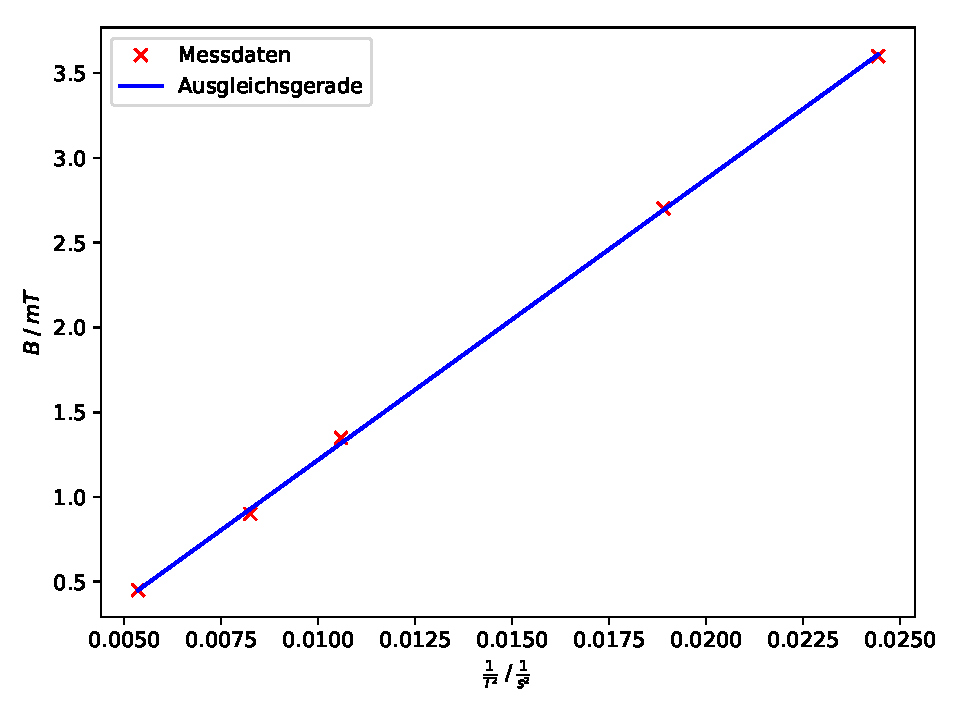
\includegraphics[scale=0.8]{content/plot1.pdf}
  \caption{Reziproke quadratische Periodendauer in Abhängigkeit vom Magnetfeld}
  \label{fig:plot1}
\end{figure}

Für die daraus folgenden Daten wird ein linearer Fit an die Funktion

\begin{equation*}
y = m_\text{fit}x+b
\end{equation*}

erstellt. 

Für die Regressionsparameter ergeben sich die Werte:

\begin{align*}
m_\text{fit} &= \SI{0.16559+-0.00294}{\kilo\gram\per\ampere},\\
b &= \SI{-0.437+-0.045}{\tesla}.
\end{align*}

Anhand von Gleichung \eqref{eqn:PeriodeM} lässt sich das magnetische Moment $m$ jetzt identifizieren als 

\begin{equation*}
m = \frac{4\theta\pi}{m_\text{fit}}.
\end{equation*}

Somit ergibt sich der Wert: 

\begin{equation*}
m = \SI{0.01019+-0.00018}{\ampere\meter²}.
\end{equation*}